\documentclass{article}

\usepackage{graphicx}

\author{Nic Hollingum - 308193415}
\title{Computational Geometry - Assignment 3}

\begin{document}
\maketitle

\section {Voronoi and Trapezoid}

\begin{figure}[htb]
\begin{center}
\leavevmode
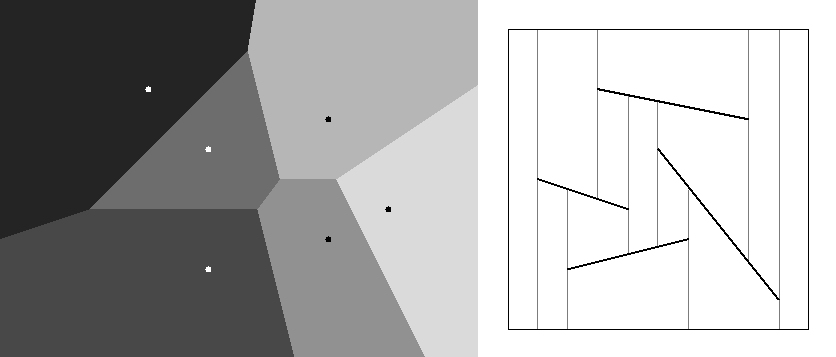
\includegraphics[width=0.9\textwidth]{voronoi.png}
\end{center}
%\caption{Voronoi Segmentation and Trapezoidal Mapping}
\label{fig:vortrap}
\end{figure}

\subsection{a) Voronoi}
A voronoi diagram divides the plane into segments (cells) around the n control points such that any point in $n_i$'s cell is closer to $n_i$ than any other control point.
For large instances, Fortune's algorithm is recommended, which uses a sweep-line technique and runs in $n log n$ time.
However with small instances (such as this) drawing by hand is not so complicated.

A simple way of drawing such a diagram by hand is to mark relative neighbours on the graph and draw a point exactly between them, then extend all points perpendicular to the relative neighbour edge at the same speed.
This particular rendering was done in java where:
\begin{itemize}
	\item for each pixel (x,y).
	\item exhaustively search the points for the closest one.
	\item colour (x,y) with that point's colour.
\end{itemize}

\subsection{b) Trapezoid}
Note, the assignment description sats the 3rd segment lies on $(5,6) \rightarrow (1,9)$, however in the picture it appears (despite being annotated otherwise) to lie on $(5,6) \rightarrow (9,1)$.
We shall go with what the picture says.

This mapping contains 13 trapezoids.
A Trapezoidal Mapping is formed by extending a line up and down at the endpoints of each segment until we reach either the bounding box or another segment.
For simplicity, and indeed in this case, we presume no 2 points share the same x coordinte.

\section {Colinear Points}

\section {Populous Cities}

\section {Trapezoidal Map Size}

We use a plane sweep to count the nuber of trapezoids behind the sweep-line.
Or more acurately, the number of trapezoids behind a sweep line $\epsilon$ distance infront of the current line.
For now we presume no 2 endpoints share an x coordinate and no segments overlap.

When we start the sweep-line , we have 1 trapezoid ``behind'' it, that is the left-most endpoint forms the x boud of the unbounded-negative-x trapezoid.
Note that the instant we pass this first control point we have 3 trapezoids, the one behind, and the 2 above and below this segment.
Presuming this segment ends without a new segment being encountered, we are left with 4 trapezoids, adding the last one in front of the segment which bounds the above/below trapezoids.
In this case we began with 1 trapezoid and added 3 when we encountered the new segment.
More genrally, when we encounter a new segment, we close a trapezoid and open 2 new ones.
When we reach the end of that segmet we close the 2 and open a 4th.

This holds no matter what configuration of trapezoids are already on the sweep-line.
When a start-point is reached, the trapezoid to the left of it is closed, whether this trapezoid is bounded above or below or both or neither.
At most one trapezoid will be bounded in this fashion, for more than 1 trapezoid to be bounded would require the line to extend through a segment and bound a second trapezoid, but this is not allowed.
exactly 2 new trapezoids are started as well.
The argument above follows here, except that ther are 2 trapezoids since the segment itself divides them.
Even if these trapezoids are closed before the endpoint is reached, this start-point still caused them to be added, so they are counted.
Finally, when the endpoint is reached, exactly 2 trapezoids are closed (the ones above and below the segment), and exactly one is started.
Note it doesnt matter if the 2 closed are the same as the 2 opened, we only care that there must be trapezoids above and below the segment which we may close.
Again the argument for the start-point applies here (in reverse, we cannot count a certain number going left to right then a different number going right to left).

So we note that the sweepline starts with 1 trapezoid and adds 3 for every segment it encounters, then the number of trapezoids t for n segments: $t = 3n + 1$.
This is true only with non-intersecting segments that dont share x coordinates.
If we remove the x-coordinate presumption we find that the number of trapezoids necessarily decreases or stays the same.

When x coordinates are the same, the sweep line may encounter multiple start and end points simultaneously.
For startpoints, the new trapezoid may indeed be new (as above) or it may not be, if it has already been counted by a different startpoint or as following an endpoint.
Similarly with endpoints, we see that trapezoids may be opened several times, closed several times or or opened then immediately closed.
Note that even if some x-coordinates are the same, this can  not affect the outcome if ther exists segments between them to block the double-counting of trapezoids.
All of these result in over-counting the number of trapezoids, thus we can say that if we remove the uniqueness constraint on x coordinates, the number of trapezoids $t <= 3n + 1$

\section {Arrangement Bounding}


\end{document}
